\documentclass[a4paper,11pt]{article}

\usepackage[utf8]{inputenc}

\usepackage{graphicx}
\usepackage{caption}
\usepackage{subcaption}

\usepackage{hyperref}

\usepackage{pgfplots}
\pgfplotsset{compat=1.18} 

\usepackage{minted}

\begin{document}

\title{
    \textbf{Assignment 1 Report - Critical Sections. Locks, Barriers, and Condition Variables}
}
\author{Dean Tsankov, Kacper Lisik}
\date{\today}

\maketitle

\section*{Introduction}

In this assignment, we learn how to write, build and execute a parallel program in OpenMP to show performance speedup on more than one processor as well as to find dependencies in loops and to write code such that it can correctly be executed in parallel.

\section*{Problem 1 - Compute the Sum, Min, and Max of Matrix Elements}

To begin with we are given the matrixSum-openmp.c program which we have to manipulate in order to complete the given tasks as an introduction to OpenMP directives.

\subsection*{Task description}

\begin{minted}[
frame=single,
framesep=2mm,
baselinestretch=1.2,
fontsize=\footnotesize,
breaklines,
]{text}
The purpose of this problem is to introduce us to basic OpenMP usage. The program matrixSum-openmp.c computes a sum of matrix elements in parallel using OpenMP. Develop and evaluate the following modified version of the program.
Extend the program so that in addition to the sum, it finds and prints a value and a position (indexes) of the maximum element of the matrix and a value and a position of the minimum element of the matrix. To check your solution, initialize elements of the matrix to random values. Use OpenMP constructs. Run the program on different numbers of processors and report the speedup (sequential execution time divided by parallel execution time) for different numbers of processors (up to at least 4) and different sizes of matrices (at least 3 different sizes). Run each program several (at least 5) times and use the median value for execution time. Try to provide reasonable explanations for your results. Measure only the parallel part of your program.
\end{minted}


\subsection*{Key points of solution}
OpenMp makes it very simple to turn a sequential implementation of a program into a concurrent one. The traversal loop over the matrix looks like so:

\begin{minted}[
frame=single,
framesep=2mm,
baselinestretch=1.2,
fontsize=\footnotesize,
]{c}
    (...)
    start_time = omp_get_wtime();
    #pragma omp parallel for reduction(+ : total) private(j) shared(min,max)
        for (i = 0; i < size; i++){
            for (j = 0; j < size; j++)
            {
                total += matrix[i][j];
                if (matrix[i][j] < min.value)
                {
                    min.value = matrix[i][j];
                    min.xCoordinate = j;
                    min.yCoordinate = i;
                }
                else if (matrix[i][j] > max.value)
                {
                    max.value = matrix[i][j];
                    max.xCoordinate = j;
                    max.yCoordinate = i;
                }
            }
        }
        // implicit barrier

        end_time = omp_get_wtime();
    (...)
\end{minted}

\subsection*{Performance exploration}

Sequential time as a median from 100 executions: \[ 8.73899 * 10^{-8}s\]

\begin{figure}[H]
    \centering
    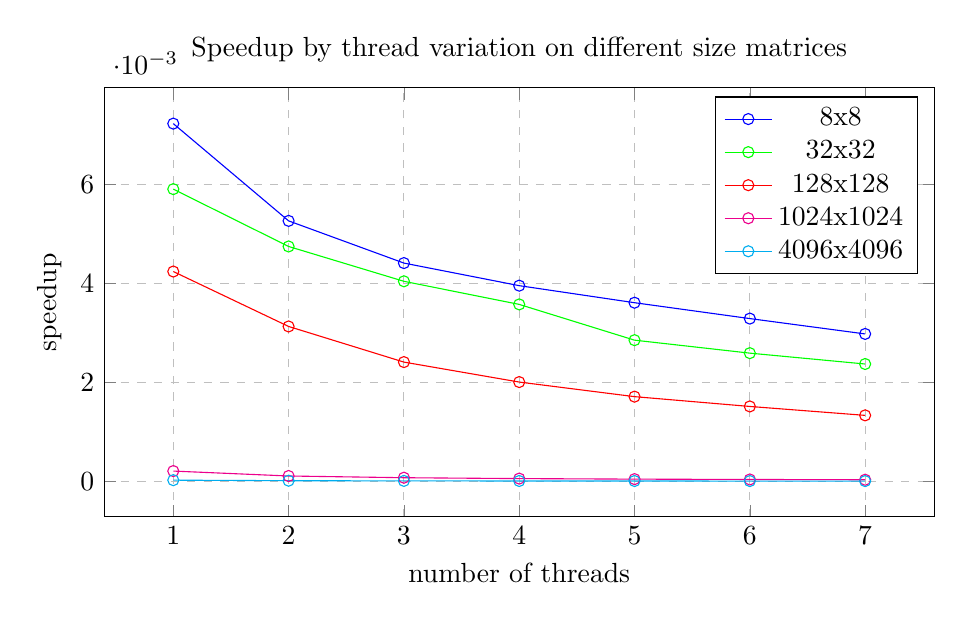
\begin{tikzpicture}
        \begin{axis}[
            title={Speedup by thread variation on different size matrices},
            width=\linewidth,
            height=200,
            xlabel={number of threads},
            ylabel={speedup},
            ymajorgrids=true,
            xmajorgrids=true,
            grid style=dashed,
        ]
        
        \addplot[
            color=blue,
            mark=o,
            ]
            coordinates {
            (1, 0.00722852)(2, 0.00526292)(3, 0.00440972)(4, 0.0039533)(5, 0.00360869)(6, 0.00328779)(7, 0.0029776)
            };
            \addlegendentry{8x8}

        \addplot[
            color=green,
            mark=o,
            ]
            coordinates {
            (1, 0.00590448)(2, 0.00474545)(3, 0.00404135)(4, 0.00357436)(5, 0.00285155)(6, 0.00258929)(7, 0.00236971)
            };
            \addlegendentry{32x32}

        \addplot[
            color=red,
            mark=o,
            ]
            coordinates {
            (1, 0.00423888)(2, 0.00312863)(3, 0.00240844)(4, 0.0020048)(5, 0.00170995)(6, 0.00151171)(7, 0.00133168)
            };
            \addlegendentry{128x128}

        \addplot[
            color=magenta,
            mark=o,
            ]
            coordinates {
            (1, 0.000205602)(2, 0.000106047)(3, 7.12769e-05)(4, 5.35315e-05)(5, 4.26937e-05)(6, 3.57209e-05)(7, 3.05576e-05)
            };
            \addlegendentry{1024x1024}

        \addplot[
            color=cyan,
            mark=o,
            ]
            coordinates {
            (1, 2.18081e-05)(2, 1.08985e-05)(3, 7.23905e-06)(4, 5.4152e-06)(5, 4.33902e-06)(6, 3.61736e-06)(7, 3.10179e-06)
            };
            \addlegendentry{4096x4096}
        \end{axis}
        \end{tikzpicture}
    \caption{Tree add time complexity}
    \label{fig:plot1}
\end{figure}

We would expect the speedup to increase not decrease. Still these results could make sense considering that parallelizing helps for big workloads, or when the workers are used many times for many moderate sized tasks (so the cost of launching the threads is a fraction of the work they do). But in this case performing comparatively small amount of additions and comparisons is negligible to a CPU. And so are just not doing enough to benefit from parallelizing this specific task.


\section*{Problem 2 - Quicksort}

\subsection*{Task description}

\begin{minted}[
frame=single,
framesep=2mm,
baselinestretch=1.2,
fontsize=\footnotesize,
breaklines,
]{text}
The quicksort algorithm sorts the list of numbers by first dividing the list into two sublists so that all the numbers if one sublist are smaller than all the numbers in the other sublist. This is done by selecting one number (called a pivot) against which all other numbers are compared: the numbers which are less than the pivot are placed in one sublist, and the numbers which more than the pivot are placed in another sublist. The pivot can be either placed in one sublist or withheld and placed in its final position. Develop a parallel multithreaded program (in C/C++ using OpenMP tasks) with recursive parallelism that implements the quicksort algorithm for sorting an array of n values. Perform speedup tests on the parallel part of the code and give explinations.
\end{minted}

\subsection*{Key points of solution}

\end{document}